\documentclass[ignorenonframetext, professionalfonts, hyperref={pdftex, unicode}]{beamer}

\usetheme{Copenhagen}
\usecolortheme{wolverine}

%Packages to be included
%\usepackage{graphicx}

\usepackage[russian]{babel}
\usepackage[utf8]{inputenc}
\usepackage[T1]{fontenc}

%%\usepackage[orientation=landscape, size=custom, width=16, height=9.75, scale=0.5]{beamerposter}

\usepackage{textcomp}

\usepackage{beamerthemesplit}

\usepackage{ulem}

\usepackage{verbatim}

\usepackage{ucs}


\usepackage{listings}
\lstloadlanguages{bash}

\lstset{escapechar=`,
	extendedchars=false,
	language=sh,
	frame=single,
	tabsize=2, 
	columns=fullflexible, 
%	basicstyle=\scriptsize,
	keywordstyle=\color{blue}, 
	commentstyle=\itshape\color{brown},
%	identifierstyle=\ttfamily, 
	stringstyle=\mdseries\color{green}, 
	showstringspaces=false, 
	numbers=left, 
	numberstyle=\tiny, 
	breaklines=true, 
	inputencoding=utf8,
	keepspaces=true,
	morekeywords={u\_short, u\_char, u\_long, in\_addr}
	}

\definecolor{darkgreen}{cmyk}{0.7, 0, 1, 0.5}

\lstdefinelanguage{diff}
{
    morekeywords={+, -},
    sensitive=false,
    morecomment=[l]{//},
    morecomment=[s]{/*}{*/},
    morecomment=[l][\color{darkgreen}]{+},
    morecomment=[l][\color{red}]{-},
    morestring=[b]",
}

\author[Epam]{{\bf Epam}\\Low Level Programming Department}

%\institution[EPAM]{EPAM}
%\logo{\includegraphics[width=1cm]{logo.png}}


\title[RPM]{Пакетирование в ОС Linux\\на примере RPM}

\begin{document}


%%%%%%%%%%%%%%%%%%%%%%%%%%%%%%%%%%%%%%%%%%%%%%%%%
%%%%%%%%%% Begin Document  %%%%%%%%%%%%%%%%%%%%%%
%%%%%%%%%%%%%%%%%%%%%%%%%%%%%%%%%%%%%%%%%%%%%%%%%

\begin{frame}
	\frametitle{}
	\titlepage
	\vspace{-0.5cm}
	\begin{center}
	%\frontpagelogo
	\end{center}
\end{frame}

\begin{frame}
	\tableofcontents
%	[hideallsubsections]
\end{frame}



%%%%%%%%%%%%%%%%%%%%%%%%%%%%%%%%%%%%%%%%%
%%%%%%%%%% Content starts here %%%%%%%%%%
%%%%%%%%%%%%%%%%%%%%%%%%%%%%%%%%%%%%%%%%%

\section{Введение}
\mode<all>{\begin{frame}{Система управления пакетами: для чего это нужно}
\begin{itemize}
 \item ''DLL Hell''
 \item Dependency hell
 \item Общие задачи пакетного менеджера:
   \begin{itemize}
     \item Проверка целостности пакетов
     \item Проверка зависимостей пакетов
        \item Поддержание списка установленных пакетов
        \item Автоматическое удаление пакетов
     \item Предоставление доступа к репозиторию пакетов
     \item Разрешение зависимостей
   \end{itemize}
\end{itemize}
\end{frame}

\begin{frame}{Debian-based и RedHat-based системы управления пакетами}
\begin{center}
 \textbf{Два уровня пакетных менеджеров}
\end{center}
\begin{columns}
  \column{0.4\textwidth}
  \begin{center}
    \textbf{RedHat-based}
  \end{center}
  \begin{itemize}
    \item dnf/yum
    \item rpm
  \end{itemize}
  \column{0.4\textwidth}
  \begin{center}
    \textbf{Debian-based}
  \end{center}
  \begin{itemize}
    \item aptitude, apt, synaptic
    \item dpkg
  \end{itemize}
\end{columns}
\end{frame}
}

\mode<all>{\begin{frame}{Структура пакета}
	\begin{itemize}
		\item Метаданные
			\begin{itemize}
				\item Имя
				\item Версия/Релиз
				\item Описание
				\item ...
			\end{itemize}
		\item Зависимости
			\begin{itemize}
				\item От чего зависят
				\item Что предоставляют
			\end{itemize}
		\item Архив с файлами
			\begin{itemize}
				\item RPM: cpio
				\item dpkg: сжатый tar
			\end{itemize}
		\item Скрипты
			\begin{itemize}
				\item Pre Install
				\item Post Install
				\item Pre Uninstall
				\item Post Uninstall \bigskip
				\item Опционально: Triggers
			\end{itemize}
	\end{itemize}
\end{frame}

\begin{frame}{''Пакетные'' дистрибутивы: зависимости}
    \begin{columns}
        \column{0.5\textwidth}
            \Large\center{Правильные пакетные зависимости}
            \center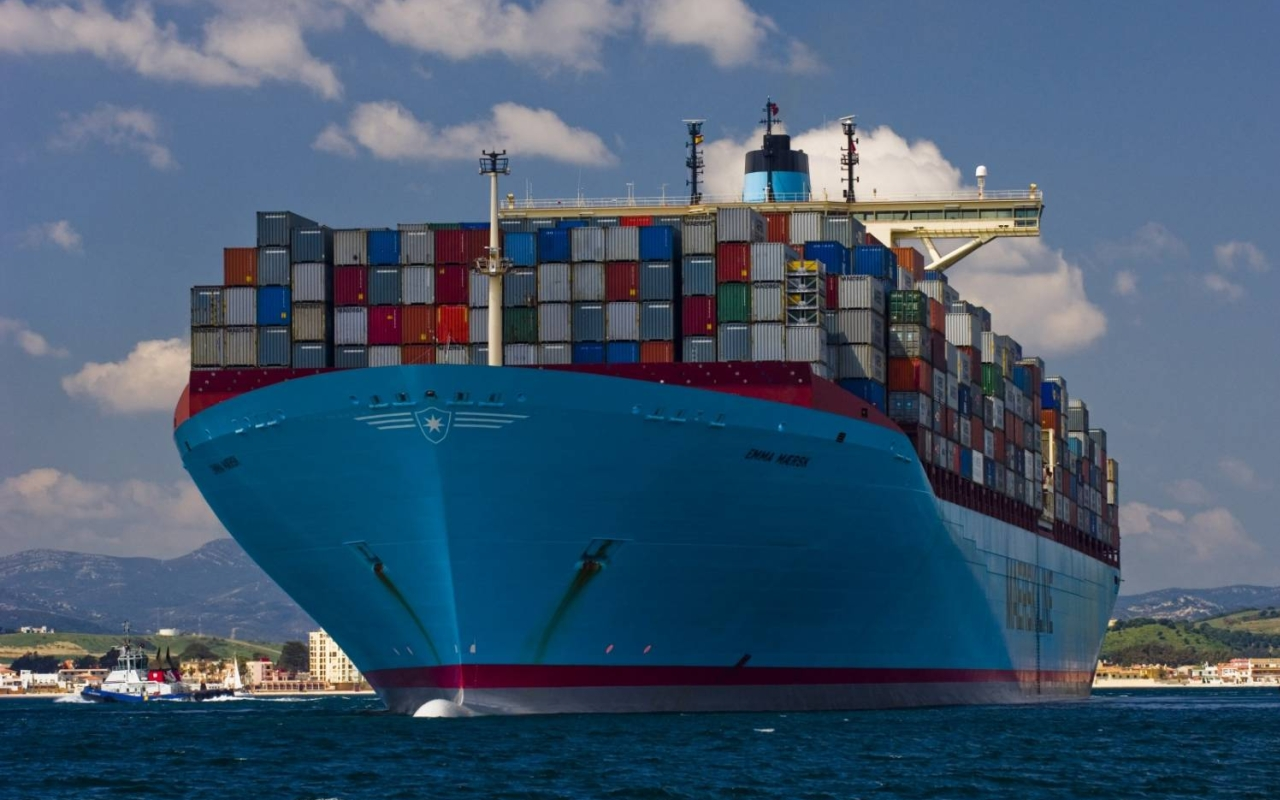
\includegraphics[width=1\textwidth]{../../slides/packaging/good-packaging.jpg}
        \column{0.5\textwidth}
            \Large\center{''Кривые'' пакетные зависимости}
            \center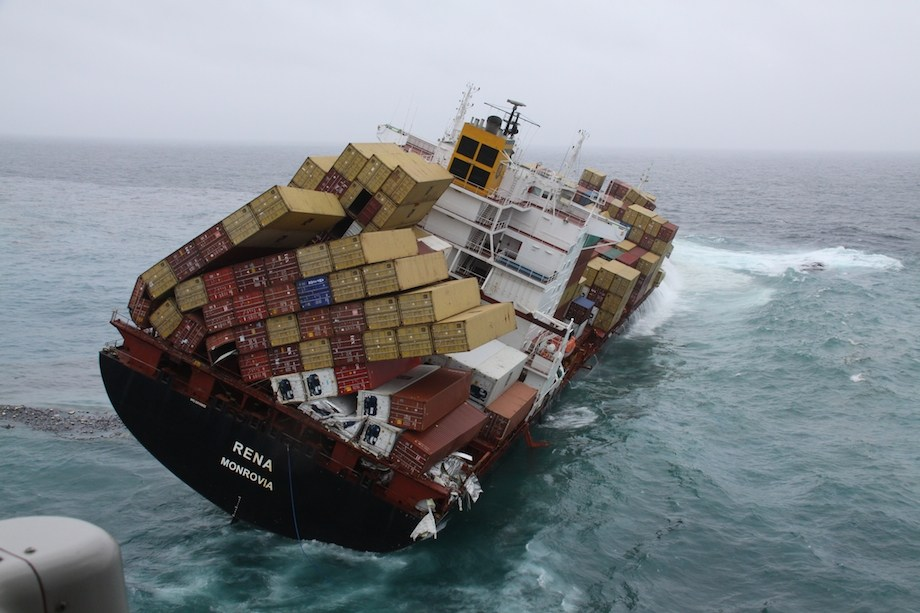
\includegraphics[width=1\textwidth]{../../slides/packaging/wrong-packaging.jpg}
    \end{columns}
\end{frame}
}

\section{RPM}
\mode<all>{\begin{frame}
%damn tilde, best that i found
\def~{$\sim$}
	\frametitle{Подготовка окружения для сборки}	
			\begin{itemize}
				\item {\tt rpmdevtools} -- разные полезные помощники
				\item {\tt rpmdev-setuptree} -- создает структуру каталогов
				\item {\tt ~/.rpmmacros} -- информация о пакетировщике, локальные
			\end{itemize}			
				\begin{table}
					\begin{tabular}{l | l | l }
					Каталог & Макрос & Описание\\
					\hline
					~/RPM/SPECS/ & \%\_specdir & Сборочные .spec файлы\\
					~/RPM/SOURCES/ & \%\_sourcedir & Исходные архивы и патчи\\
					\hline
					~/RPM/BUILD/ & \%\_builddir	& Сборка\\		
					~/RPM/BUILDROOT/ & \%\_buildrootdir & Установка\\
					\hline
					~/RPM/RPMS/ & \%\_rpmdir & Собранные .rpm\\
					~/RPM/SRPMS/ & \%\_srcrpmdir & ``Собранный'' .srpm \\
					\end{tabular}
				\end{table}			
\end{frame}

\begin{frame}
\def~{$\sim$}
\frametitle{Пример 0: Hello, World!}

	\begin{block}{Упражнение: hello.spec}
		\begin{itemize}
			\item Скопировать файл описания сборки {\tt hello.spec} в {\tt ~/RPM/SPECS/}
			\item Скопировать файл c исходным кодом в {\tt ~/RPM/SOURCES/}
			\item Собрать пакет с помощью {\tt rpmbuild -ba ~/RPM/SPECS/hello.spec}
			\item Посмотреть получившуюся файловую структуру {\tt find ~/RPM/}
		\end{itemize}
	\end{block}

\end{frame}

\begin{frame}
	\frametitle{Шаги сборки}
	
			\begin{table}
				\begin{tabular}{l | l | l | l }
				Шаг & Чтение & Запись & Описание \\
				\hline 
				\%prep & \%\_sourcedir & \%\_builddir & Подготовка\\
				\%build & \%\_builddir & \%\_builddir & Сборка (configure, make)\\
				\%install & \%\_builddir & \%\_buildrootdir & Установка (make install)\\
				\%check &	\%\_builddir & \%\_builddir & Проверка (make test)\\
				\hline 
				bin & \%\_buildrootdir	&\%\_rpmdir & Упаковка RPM\\
				src & \%\_sourcedir & \%\_srcrpmdir & Упаковка SRPM\\
				\end{tabular}
			\end{table}
\end{frame}

\begin{frame}
	\frametitle{Структура spec-файла}
	\begin{itemize}
		\item Тэги -- {\tt Tag: value}
		\begin{itemize}
		\item Все из открытого шаблона .spec файла
		\item Отсутствующие в шаблоне
			\begin{itemize}
			\item {\tt Patch0: } имя файла с патчем
			\item {\tt BuildArch/ExcludeArch/ExclusiveArch: } архитектура (noarch)
			\item {\tt BuildRoot: } BUILDROOT каталог устарело
			\end{itemize}
		\item Зависимости
			\begin{itemize}
			\item {\tt BuildRequires:}
			\item {\tt Requires:}
			\item {\tt Provides:}
			\item {\tt Conflicts:}
			\item {\tt Obsoletes:}
			\item {\tt AutoReqProv: (0|1)}
			\end{itemize}
		\end{itemize}
	\end{itemize}
\end{frame}

\begin{frame}
	\frametitle{Структура spec-файла}

	\begin{itemize}
		\item Секции --  {\tt \%prep, \%build, \%install, \%check, \%files, \%changelog} 
		\item Макросы -- {\tt \%define FOO bar} 
		\item Скриптлеты, выполняемые в различных условиях\\
			{\tt (pre-,post-)install, uninstall, trigger}
		\item Подпакеты -- {\tt \%package}
		\item Условности -- {\tt \%ifarch ARCH\_NAME, \%if TRUE\_OR\_FALSE}
	\end{itemize}
	\begin{block}{Hint:}
		 {\tt rpm -\-showrc }
	\end{block}
\end{frame}

\begin{frame}
	\frametitle{Пример 1: Hello, World!}

	\begin{block}{Упражнение: hello.spec}
		\begin{itemize}
			\item Собрать пакет с помощью {\tt rpmbuild -ba hello.spec}
			\item Посмотреть список зависимостей {\tt rpm -qRp hello*.rpm}
			\item Установить полученный пакет
			\begin{itemize}
				\item {\tt apt-cache dotty template > template.dot}
				\item {\tt dot -Tpng template.dot -o template.png}
			\end{itemize}
			\item Удалить исходники и spec-файл
			\item Пересобрать пакет из SRPM {\tt rpmbuild -{}-rebuild *.src.rpm}
		\end{itemize}
	\end{block}

	\pause

	\begin{block}{Упражнение: расширяем функционал}
		Добавить компиляцию, установку и пакетирование для CPP-примера.
	\end{block}

\end{frame}


\begin{frame}
	\frametitle{Разработка и использование в реальной системе}
	
	\begin{block}{Build-time vs Run-time}

		\begin{enumerate}
			\item Не все, что нужно во время компиляции, должно быть установлено в конечной системе.
			\item Не все, что нужно для работы программы, необходимо устанавливать на сборочной системе.
		\end{enumerate}
	\end{block}
	\begin{block}{Чистое сборочное окружение}
		\begin{itemize}
			\item Воспроизводимость сборки 
			\item Контроль зависимостей
			\item Контроль автоматически "подхваченных" зависимостей
		\end{itemize}
	\end{block}
\end{frame}

\begin{frame}
	\frametitle{Версии}

	\Large{Чтение правил дистрибутива строго обязательно!}
	
	Hint: {\tt rpmdev-vercmp (rpmdevtools)}
	\begin{block}{ Версия -- составная}
		{\tt \%name-\%epoch:\%version-\%release}
		\begin{itemize}
			\item {\tt Name: == \%name}
			\item {\tt Epoch: == \%epoch}
			\item {\tt Version: == \%version}
			\item {\tt Release: == \%release}
			\begin{itemize}
				\item Release:
				\item \%\{?dist\} tag
				\item rebuild number -- автоматически (при использовании нормальных билд-систем)
			\end{itemize}
		\end{itemize}
	\end{block}

\end{frame}


\begin{frame}
	\frametitle{Пример 2}

	\begin{block}{Подпакеты, скрипты, зависимости и обновление}
		На примере {\tt template.spec}:

		\begin{itemize}
			\item Собрать пакет с помощью {\tt rpmbuild -ba template.spec}
			\item Посмотреть список зависимостей {\tt rpm -qRp template*.rpm}
			\item Установить полученные пакеты
			\item Изменить версию, пересобрать и обновить в системе
			\item Построить дерево зависимостей:
			\item Удалить полученные пакеты
		\end{itemize}
	\end{block}
\end{frame}

\begin{frame}
	\frametitle{Задача на дом: Пакетируем linking}

	\begin{block}{Задача:}
		Создать и установить пакеты для примера с созданием библиотек
		и их использования из предыдущих лекций.
	\end{block}

	Hint: libtestA, libtestB, libtestA-devel, libtestB-devel, mainpkg

\end{frame}

}

\mode<all>\begin{frame}[fragile]{Вопросы?}
    \setcounter{tocdepth}{2}
    \tableofcontents

    \bigskip

    \hrulefill
    \begin{columns}
    \column{0.7\textwidth}
            \center{Материалы:}
            \url{https://yadi.sk/d/Ixp8kHfl3MipCq}
    \column{0.2\textwidth}
        \begin{center}
            
\includegraphics[width=0.7\textwidth]{url-qr-2017}
        \end{center}
    \end{columns}

    Исходники: \url{https://github.com/epam-llpd/linux_courses}

\end{frame}

\end{document}
